% !TEX root = task-1-16-1.tex
% Editable task bank. Append new BankTask blocks at the end of the document.
\documentclass[12pt,a4paper]{article}
\usepackage{physics-textbook}
\usepackage{graphicx,needspace}
\usetikzlibrary{decorations.pathmorphing}
\newif\ifShowSolutions
\ifdefined\TutorEdition
  \ShowSolutionstrue
\else
  \ShowSolutionsfalse % Change to \ShowSolutionstrue to display solutions.
\fi
\newcounter{banktask}
\newsavebox{\BankTaskBox}
\newcommand{\BankTaskContent}[3]{%
  \noindent\textbf{\thebanktask.}\quad #2\par
  \ifShowSolutions
    \Needspace{50mm}% Keep the solution heading with its opening text or diagram.
    #3\par
    \ifdefined\TutorEdition
      \ifcsname TutorSource#1\endcsname
        \nopagebreak\smallskip{\small\csname TutorSource#1\endcsname\par}%
      \fi
    \fi
  \fi
}
\newcommand{\BankTask}[3]{%
  \refstepcounter{banktask}\par\medskip
  \sbox{\BankTaskBox}{\begin{minipage}{\linewidth}%
    \BankTaskContent{#1}{#2}{#3}\end{minipage}}%
  \ifdim\dimexpr\ht\BankTaskBox+\dp\BankTaskBox\relax>\dimexpr\textheight-20mm\relax
    \Needspace{35mm}\BankTaskContent{#1}{#2}{#3}%
  \else
    \Needspace{\dimexpr\ht\BankTaskBox+\dp\BankTaskBox\relax}%
    \noindent\usebox{\BankTaskBox}\par
  \fi
  \medskip
}
\begin{document}
\BookSubsection{1.16.1}{Рычаг}


% Source sdamgia-26715: https://phys-ege.sdamgia.ru/problem?id=26715
\BankTask{sdamgia-26715}{
На рычаг действуют две силы. Момент первой силы относительно оси вращения рычага равен $50\,\text{Н}\cdot\text{м}$. Какова величина второй силы, если ее плечо относительно этой же оси равно $0{,}5 \,\text{м}$ и рычаг при этом находится в равновесии?
}{
\smallskip\noindent\textbf{Решение}\par
Так как рычаг находится в равновесии, то по правилу моментов $M_{1}=M_{2} .$ Момент второй силы равен $M_{2} =F_{2} \cdot d_{2} .$ Откуда находим величину второй силы:

$F_{2} = \frac{ M_{2} }{ d_{2} } = \frac{ 50\,\text{Н} \cdot \,\text{м}}{ 0{,}5\,\text{м} } =100\,\text{Н}.$

Ответ: $100$.
}

% Source sdamgia-35321: https://phys-ege.sdamgia.ru/problem?id=35321
\BankTask{sdamgia-35321}{
\begin{center}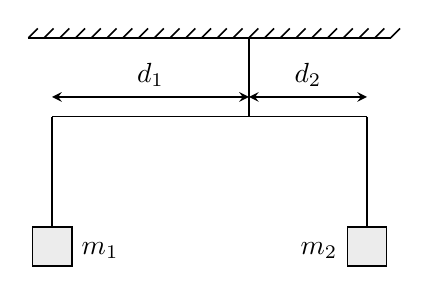
\begin{tikzpicture}[x=1cm,y=1cm,>=stealth,line width=.55pt]
\draw (-.3,2.7)--(4.3,2.7);\foreach \x in {-.3,-.1,...,4.3}{\draw(\x,2.7)--++(.12,.12);}\draw(2.5,2.7)--(2.5,1.7);\draw(0,1.7)--(4,1.7);\draw(0,1.7)--(0,.3);\draw(4,1.7)--(4,.3);\draw[fill=gray!15](-.25,-.2)rectangle(.25,.3);\draw[fill=gray!15](3.75,-.2)rectangle(4.25,.3);\node[right]at(.25,0){$m_1$};\node[left]at(3.75,0){$m_2$};\draw[<->](0,1.95)--(2.5,1.95)node[midway,above]{$d_1$};\draw[<->](2.5,1.95)--(4,1.95)node[midway,above]{$d_2$};
\end{tikzpicture}\end{center}
Коромысло весов, к которому подвешены на нитях два груза (см. рис.), находится в равновесии. Массу первого груза увеличили в $2$ раза. Во сколько раз нужно уменьшить плечо $d_{1}$, чтобы равновесие сохранилось? (Коромысло и нити считать невесомыми.)
}{
\smallskip\noindent\textbf{Решение}\par
Рычаг находится в равновесии, если моменты приложенных сил равны. Поскольку плечо второй силы и массу второго груза не меняли, то момент этой силы не изменился. Соответственно, момент первой силы также остался прежним. Поскольку момент силы равен $M=m_{1}gd_{1},$ масса груза увеличилась в $2$ раза, то плечо силы необходимо уменьшить в $2$ раза.
 
Ответ: $2$.
}

% Source sdamgia-35987: https://phys-ege.sdamgia.ru/problem?id=35987
\BankTask{sdamgia-35987}{
К концу тонкого жесткого однородного стержня длиной $50 \,\text{см}$ и массой $300 \,\text{г}$ прикреплен маленький шарик массой $200 \,\text{г}$. На каком расстоянии от шарика нужно поставить под него тонкую опору, чтобы эта система тел находилась в равновесии в однородном поле силы тяжести?
}{
\smallskip\noindent\textbf{Решение}\par
Рычаг находится в равновесии, если моменты приложенных сил равны. Пусть плечо силы, действующей на рычаг со стороны шарика, равно $x$. Тогда плечо силы тяжести однородного стрежня равно $\frac{ l}{ 2 } - x.$ По правилу моментов рычаг находится в равновесии, если выполняется условие:

$mg ( \frac{ l}{ 2 } - x ) = m_{1}gx,$

откуда находим расстояние от точки опоры до маленького шарика:

$x= \frac{ ml}{ 2 ( m + m_{1} ) } = \frac{ 300 \cdot 50}{ 2 ( 300 + 200 ) } =15\,\text{см}.$

Ответ: $15$.
}

% Source sdamgia-10176: https://phys-ege.sdamgia.ru/problem?id=10176
\BankTask{sdamgia-10176}{
К горизонтальной легкой рейке, лежащей на двух опорах А и В, в точке О прикреплен груз массой $10 \,\text{кг}$. Длина отрезка ОА равна $4 \,\text{м}$, длина отрезка ОВ равна $1 \,\text{м}$. Определите модуль силы, с которой действует на рейку опора В.

\begin{center}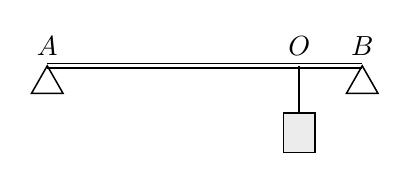
\begin{tikzpicture}[x=1cm,y=1cm,>=stealth,line width=.55pt]
\draw[double,double distance=1pt] (0,0)--(4,0);\draw (0,0)--(-.2,-.35)--(.2,-.35)--cycle;\draw (4,0)--(3.8,-.35)--(4.2,-.35)--cycle;\node[above] at(0,0){$A$};\node[above] at(4,0){$B$};\node[above] at(3.2,0){$O$};\draw (3.2,0)--(3.2,-.6);\draw[fill=gray!15] (3,-1.1) rectangle (3.4,-.6);
\end{tikzpicture}\end{center}
}{
\smallskip\noindent\textbf{Решение}\par
На рейку действуют сила реакции опоры в точке $A$ и в точке $B$, а также сила тяжести груза. Запишем уравнение моментов относительно точки А:

$mg \cdot OA=N_{B} \cdot AB \Rightarrow N_{B} = \frac{ mg \cdot OA}{ AB } = \frac{ 10 \cdot 10 \cdot 4}{ 5 } =80\,\text{Н}.$

Ответ: $80$.
}

% Source sdamgia-27082: https://phys-ege.sdamgia.ru/problem?id=27082
\BankTask{sdamgia-27082}{
Тяжелая однородная рейка может вращаться вокруг горизонтальной оси, проходящей через точку О (см. рис.).

\begin{center}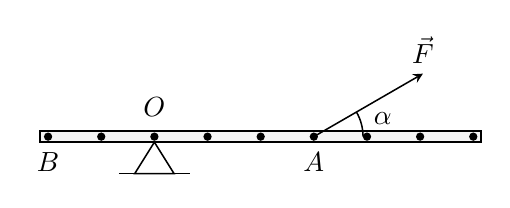
\begin{tikzpicture}[x=1cm,y=1cm,>=stealth,line width=.55pt]
\draw[fill=gray!8] (0,0) rectangle (5.6,.14);\foreach \i in {0,...,8}{\fill (.1+.675*\i,.07) circle(1.5pt);}\draw (1.45,0)--(1.2,-.4)--(1.7,-.4)--cycle;\draw (1,-.4)--(1.9,-.4);\node[above] at (1.45,.2){$O$};\node[below] at (.1,0){$B$};\node[below] at (3.475,0){$A$};\draw[->] (3.475,.07)--++(30:1.6) node[above]{$\vec F$};\draw (4.1,.07) arc(0:30:.625);\node at (4.35,.3){$\alpha$};
\end{tikzpicture}\end{center}

В рейке проделаны небольшие отверстия (они показаны на рисунке черными точками). Расстояние между соседними отверстиями $8 \,\text{см}$. С помощью силы $F=10 \,\text{Н}$, приложенной в точке А и направленной под углом $\alpha =30 ^\circ$ к рейке, она удерживается в равновесии. Чему равен модуль момента силы $F$ относительно горизонтальной оси, проходящей через точку $B$?
}{
\smallskip\noindent\textbf{Решение}\par
Плечо силы $F$ относительно точки В равно $d=5 \cdot 0{,}08 \cdot \sin 30 ^\circ =0{,}2\,\text{м}.$ Тогда момент силы относительно точки В найдем по формуле $M=F \cdot d=10\,\text{Н} \cdot 0{,}2\,\text{м}=2\,\text{Н} \cdot \,\text{м}.$
 
Ответ: $2$.
}

% Source sdamgia-10309: https://phys-ege.sdamgia.ru/problem?id=10309
\BankTask{sdamgia-10309}{
К легкой рейке подвешено на нити тело массой $7 \,\text{кг}$ (см. рис.). Рейка уравновешена на шероховатой опоре в горизонтальном положении с помощью силы $\vec{F},$ приложенной к концу рейки и направленной под углом $\alpha=30 ^\circ$ к горизонту. Определите модуль вертикальной составляющей силы реакции опоры, действующей на рейку в точке $O$.

\begin{center}\begin{tikzpicture}[x=1cm,y=1cm,>=stealth,line width=.55pt]
\draw[double,double distance=1pt] (0,0)--(5.6,0);\foreach \i in {0,...,14}{\fill (.4*\i,0) circle(1pt);}\draw (2.8,0)--(2.6,-.35)--(3,-.35)--cycle;\node[above] at(2.8,.1){$O$};\draw (1.6,0)--(1.6,-.7);\draw[fill=gray!15] (1.4,-1.15) rectangle (1.8,-.7);\node[below] at(1.6,-1.15){$7\,\text{кг}$};\draw[->] (0,0)--(-1,.58) node[above]{$\vec F$};\draw (-.6,0) arc(180:150:.6);\draw(-.9,0)--(0,0);\node at(-.7,.2){$\alpha$};
\end{tikzpicture}\end{center}
}{
\smallskip\noindent\textbf{Решение}\par
Так как рейка уравновешена, запишем правило моментов относительно левого края рейки, тем самым исключив силу $F$:

$Nd_{1}=mgd_{2} \Longleftrightarrow N= \frac{ mgd_{2}}{ d_{1} } = \frac{ 70 \cdot 4}{ 7 } =40\,\text{Н}.$

Ответ: $40$.
}

% Source sdamgia-26733: https://phys-ege.sdamgia.ru/problem?id=26733
\BankTask{sdamgia-26733}{
\begin{center}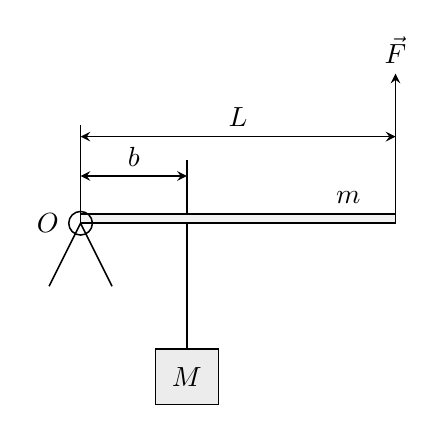
\begin{tikzpicture}[x=1cm,y=1cm,>=stealth,line width=.55pt]
\draw[fill=gray!10] (0,0) rectangle (4,.12);\draw (0,0) circle (.15);\draw (-.4,-.8)--(0,0)--(.4,-.8);\draw[<->] (0,1.1)--(4,1.1) node[midway,above]{$L$};\draw (0,.12)--(0,1.25);\draw (4,.12)--(4,1.4);\draw[<->] (0,.6)--(1.35,.6) node[midway,above]{$b$};\draw (1.35,.12)--(1.35,.8);\draw[->] (4,0)--(4,1.9) node[above]{$\vec F$};\node[left] at (-.15,0){$O$};\node[above] at (3.4,.12){$m$};\draw (1.35,0)--(1.35,-1.6);\draw[fill=gray!15] (.95,-2.3) rectangle (1.75,-1.6);\node at (1.35,-1.95){$M$};
\end{tikzpicture}\end{center}
Груз массой $M=75 \,\text{кг}$ медленно поднимают с помощью рычага, приложив вертикальную силу $\vec{F}$ (см. рис.). Рычаг, сделанный из однородного стержня массой $m=10 \,\text{кг}$ и длиной $L=4 \,\text{м}$, шарнирно закреплен. Определите модуль силы $\vec{F},$ если расстояние $b$ от оси шарнира до точки подвеса груза равно $1{,}6 \,\text{м}$. Считать, что трение в шарнире отсутствует.
}{
\smallskip\noindent\textbf{Решение}\par
\begin{center}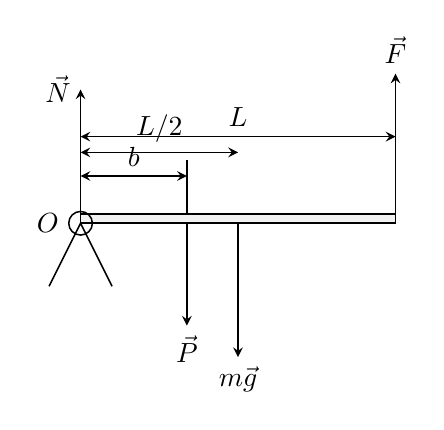
\begin{tikzpicture}[x=1cm,y=1cm,>=stealth,line width=.55pt]
\draw[fill=gray!10] (0,0) rectangle (4,.12);\draw (0,0) circle (.15);\draw (-.4,-.8)--(0,0)--(.4,-.8);\draw[<->] (0,1.1)--(4,1.1) node[midway,above]{$L$};\draw (0,.12)--(0,1.25);\draw (4,.12)--(4,1.4);\draw[<->] (0,.6)--(1.35,.6) node[midway,above]{$b$};\draw (1.35,.12)--(1.35,.8);\draw[->] (4,0)--(4,1.9) node[above]{$\vec F$};\node[left] at (-.15,0){$O$};\draw[->] (1.35,0)--(1.35,-1.3) node[below]{$\vec P$};\draw[->] (2,0)--(2,-1.7) node[below]{$m\vec g$};\draw[->] (0,0)--(0,1.7) node[left]{$\vec N$};\draw[<->] (0,.9)--(2,.9) node[midway,above]{$L/2$};
\end{tikzpicture}\end{center}

\par\smallskip\noindent $1$. Рассмотрим силы, действующие на рычаг (см. рис.). 
Считая, что рычаг поднимает груз медленно и равномерно, примем, исходя из третьего и второго законов Ньютона, что $|\vec{P} |=|M \vec{g}|.$
\par\smallskip\noindent $2$. Рассмотрим равновесие рычага относительно оси вращения — шарнира О, указав плечи сил на рисунке. $O: Mg \cdot b + \frac{ 1}{ 2 } mgL - FL=0.$
Отсюда:

$F=Mg \cdot \frac{ b}{ L } + \frac{ 1}{ 2 } mg=75 \cdot 10 \cdot \frac{ 1{,}6}{ 4 } + \frac{ 1}{ 2 } \cdot 10 \cdot 10=350\,\text{Н}.$

 
Ответ: $F=350 \,\text{Н}$.
}

% Source sdamgia-25401: https://phys-ege.sdamgia.ru/problem?id=25401
\BankTask{sdamgia-25401}{
Деревянная линейка длиной $l=90 \,\text{см}$ выдвинута за край стола на $\frac{ 1}{ 4 }$ часть своей длины. При этом она не опрокидывается, если на ее правом конце лежит груз массой не более $m_{1}=250\,\text{г}.$ Далее линейку выдвинули вправо за край стола на некоторое расстояние и положили на ее правый конец груз массой $m_{2}=125\,\text{г}.$ На какое расстояние дополнительно можно выдвинуть линейку во втором опыте, чтобы она не перевернулась?
}{
\smallskip\noindent\textbf{Решение}\par
На линейку в обоих случаях действую сила тяжести линейки, приложенная к ее середине и вес груза. Линейка находится в равновесии, поэтому можно записать правило моментов для каждого случая относительно точки опоры — края стола. В первом случае плечи силы тяжести линейки и веса груза равны $\frac{ l}{ 4 } .$ 
Следовательно, масса линейки равна массе груза $M=m_{1}=250\,\text{г}.$

\begin{center}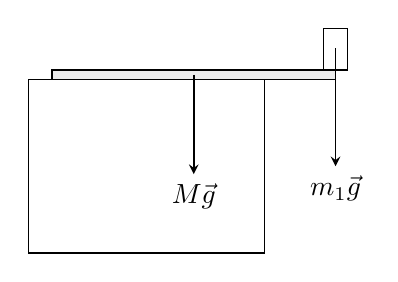
\begin{tikzpicture}[x=1cm,y=1cm,>=stealth,line width=.55pt]
\draw (0,-2.2) rectangle (3,0);\draw[fill=gray!15] (0.3,0) rectangle (3.9,.12);\draw[fill=white] (3.75,.12) rectangle (4.05,.65);\draw[->] (2.1,.06)--(2.1,-1.2) node[below]{$M\vec g$};\draw[->] (3.9,.4)--(3.9,-1.1) node[below]{$m_1\vec g$};
\end{tikzpicture}\end{center}

\begin{center}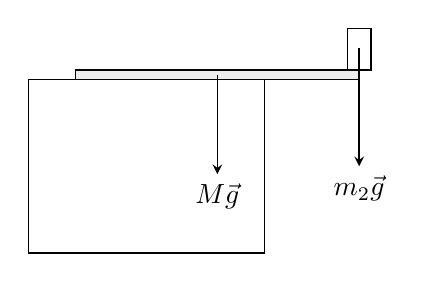
\begin{tikzpicture}[x=1cm,y=1cm,>=stealth,line width=.55pt]
\draw (0,-2.2) rectangle (3,0);\draw[fill=gray!15] (0.6,0) rectangle (4.2,.12);\draw[fill=white] (4.05,.12) rectangle (4.3500000000000005,.65);\draw[->] (2.4,.06)--(2.4,-1.2) node[below]{$M\vec g$};\draw[->] (4.2,.4)--(4.2,-1.1) node[below]{$m_2\vec g$};
\end{tikzpicture}\end{center}

Во втором случае плечо веса груза равно $l_{2}$ а плечо силы тяжести линейки $\frac{ l}{ 2 } - l_{2}.$
Запишем правило моментов для второго случая:

$m_{2}gl_{2}=Mg ( \frac{ l}{ 2 } - l_{2} ) ,$ откуда плечо веса груза:
$l_{2}= \frac{ Ml}{ 2 ( m_{2} + M ) } = \frac{ 250 \cdot 90}{ 2 \cdot ( 125 + 250 ) } =30\,\text{см}.$

Учитывая, что в первом случае расстояние равнялось $\frac{ l}{ 4 } = \frac{ 90}{ 4 } =22{,}5\,\text{см},$ линейка останется в равновесии, если ее выдвинуть на $7{,}5 \,\text{см}$.
 
Ответ: $7{,}5 \,\text{см}$.
}

% Source sdamgia-3418: https://phys-ege.sdamgia.ru/problem?id=3418
\BankTask{sdamgia-3418}{
Однородную балку поднимают за один конец, прикладывая силу $\vec{F}$ перпендикулярно балке. На рисунке показан график изменения модуля силы по мере подъема конца балки. 

 

\begin{center}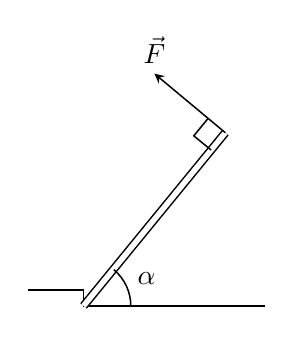
\begin{tikzpicture}[x=1cm,y=1cm,>=stealth,line width=.55pt]
\draw (-.7,0)--(0,0)--(0,-.2)--(2.3,-.2);\draw[double,double distance=2pt] (0,-.2)--(1.8,2);\draw[->] (1.8,2)--(.9,2.75) node[above]{$\vec F$};\draw (1.62,1.78)--(1.4,1.96)--(1.58,2.18);\draw (.6,-.2) arc(0:50:.6);\node at (.8,.15){$\alpha$};
\end{tikzpicture}\end{center}

\begin{center}\begin{tikzpicture}[x=1cm,y=1cm,>=stealth,line width=.55pt]
\draw[step=.5,gray!50,thin] (0,0) grid (3,3);\draw[->] (-.25,0)--(3.4,0) node[right]{$\alpha,\ \text{рад}$};\draw[->] (0,-.25)--(0,3.35) node[above]{$F,\ \text{Н}$};\draw[thick] (0,2) arc(90:0:2);\foreach \y/\v in {.5/100,1/200,1.5/300,2/400}{\node[left] at(0,\y){$\v$};}\node[below left] at(0,0){$0$};\node[below] at(2,0){$\pi/2$};
\end{tikzpicture}\end{center}

Чему равна масса балки?
}{
\smallskip\noindent\textbf{Решение}\par
Проще всего определить массу балки, рассмотрев самое начало подъема. Для того чтобы правый конец балки начал подниматься, вращающий момент, создаваемый силой $\vec{F}$ относительно левого конца балки, должен стать больше момента, создаваемого силой тяжести относительно этой точки. Сила тяжести приложена к центру масс балки. Поскольку балка однородная, ее центр масс расположен посередине. Обозначим длину балки через $L.$ По правилу моментов приложенных сил $Mg \frac{ L}{ 2 } =FL.$ 
Следовательно, масса балки равна $M= \frac{ 2F}{ g } .$ Из графика видно, что в самом начале для подъема балки была необходима сила в $400 \,\text{Н}$. Следовательно, масса балки равна $M=\frac{2\cdot400}{10}=80\,\text{кг}$.
 
Ответ: $80 \,\text{кг}$.
}

% Source sdamgia-9099: https://phys-ege.sdamgia.ru/problem?id=9099
\BankTask{sdamgia-9099}{
Однородная лестница массой $20 \,\text{кг}$ прислонена к гладкой вертикальной стене, составляя с ней угол $60^\circ$. Пол шероховатый. Чему равен модуль силы реакции, действующей на верхний конец лестницы?
}{
\smallskip\noindent\textbf{Решение}\par
\begin{center}\begin{tikzpicture}[x=1cm,y=1cm,>=stealth,line width=.55pt]
\draw[->](0,0)--(3.8,0)node[right]{$x$};\draw[->](0,0)--(0,2.5)node[above]{$y$};\draw(0,1.8)--(3.12,0);\node[below]at(3.12,0){$O$};\draw[->](0,1.8)--(1,1.8)node[above]{$\vec N_1$};\draw[->](3.12,0)--(3.12,1.1)node[right]{$\vec N_2$};\draw[->](3.12,0)--(2,0);\node[anchor=north] at (2.55,-.16){$\vec F_{\text{тр}}$};\draw[->](1.56,.9)--(1.56,-.1);\node[anchor=north east] at (1.47,-.15){$m\vec g$};\draw(0,1.2)arc(-90:-30:.6);\node at(.35,1.1){$60^\circ$};
\end{tikzpicture}\end{center}

Запишем правило моментов, взяв за ось вращения точку $O$, а за длину лестницы $l$:

$N_{1}l \cos \alpha =mg \frac{ l}{ 2 } \sin \alpha .$

Выразим модуль силы реакции, действующей на верхний конец лестницы:

$N_{1}= \frac{ mg \tan \alpha }{ 2 } = \frac{ 20 \cdot 10 \cdot \sqrt{3} }{ 2 } \approx 173\,\text{Н}.$

Ответ: $173 \,\text{Н}$.
}


% Source B0907A: https://ege.fipi.ru/bank/questions.php?search=1&proj=BA1F39653304A5B041B656915DC36B38&qid=B0907A
\BankTask{B0907A}{
Ученик выполнял лабораторную работу по исследованию условий равновесия лёгкого рычага под действием двух сил. Полученные результаты он занёс в таблицу. Результат выразите в $\text{м}$.
\begin{center}\begin{tabular}{|c|c|c|c|}\hline
$F_1,\,\text{Н}$ & $l_1,\,\text{м}$ & $F_2,\,\text{Н}$ & $l_2,\,\text{м}$ \\\hline
$60$ & $?$ & $120$ & $0{,}2$ \\\hline
\end{tabular}\end{center}
Каково плечо $l_1$, если рычаг находится в равновесии?
}{
\smallskip\noindent\textbf{Решение от GPT}\par
Условие равновесия $F_1l_1=F_2l_2$. Тогда $l_1=120\cdot0{,}2/60=0{,}4\,\text{м}$.
}

% Source 0BA328: https://ege.fipi.ru/bank/questions.php?search=1&proj=BA1F39653304A5B041B656915DC36B38&qid=0BA328
\BankTask{0BA328}{
Момент первой силы, действующей на рычаг, равен $50\,\text{Н}\cdot\text{м}$. Какой должна быть вторая сила, чтобы рычаг находился в равновесии, если её плечо равно $0{,}5\,\text{м}$? Результат выразите в $\text{Н}$.
}{
\smallskip\noindent\textbf{Решение от GPT}\par
Для равновесия $F_2l_2=M_1$. Поэтому $F_2=50/0{,}5=100\,\text{Н}$.
}

\end{document}
